\clearpage
\section{Processi di supporto}
\subsection{Documentazione}
\subsubsection{Descrizione}
Verranno qui discusse le scelte intraprese per la scrittura, \markg{verifica} ed approvazione della documentazione ufficiale di \emph{duckware}. Queste norme sono obbligatorie per tutti i documenti, i quali verranno elencati nella sottosezione \emph{Documenti correnti}.
\subsubsection{Ciclo di vita della documentazione}
Qualsiasi documento dovrà passare per gli stati di “\emph{Sviluppo}”, “\emph{Verifica}” ed “\emph{Approvato}”. Nel particolare, ciascuno di questi indica una fase precisa:
\begin{itemize}
	\item \textbf{Sviluppo}: Questa fase inizia con la creazione del documento e termina con la conclusione della stesura di tutte le sue parti. In questa fase i \emph{redattori} aggiungono le parti assegnate usando i \markg{ticket};
	\item \textbf{Verifica}: Questa fase inizia dopo l’assegnazione da parte del \emph{\markg{responsabile}}. I \emph{verificatori} effettueranno i controlli necessari e, in caso di esito positivo, il documento entra automaticamente nella fase “\emph{Approvato}”. In caso di esito negativo sarà necessario che il \emph{\markg{responsabile}} di progetto riassegni il documento ad un \emph{redattore} attraverso una nuova fase di "\emph{Sviluppo}";
	\item \textbf{Approvato}: Questa fase coincide con il completamento della parte di "\emph{Verifica}" avvenuta con successo nella quale il \emph{verificatore} certifica la correttezza. Il documento verrà dunque consegnato al \emph{\markg{responsabile}} il quale lo approverà per il rilascio esterno.
\end{itemize}

\subsubsection{Separazione tra documenti interni ed esterni}
Ogni documento dovrà avere una specifica classificazione. Vi saranno sia documenti \textbf{interni} in lingua italiana che verranno utilizzati da \emph{duckware} internamente, sia documenti \textbf{esterni} che verranno condivisi con \emph{la Proponente} ed i committenti. Questi ultimi potrebbero essere scritti in lingua inglese nel caso potesse essere utile al fine di soddisfare le richieste di deploy dell’utente finale.

\subsubsection{Nomenclatura dei documenti}
Ogni documento, tranne la Lettera di Presentazione ed i Verbali, adotteranno questo schema di nomenclatura:
\begin{itemize}
	\item \textbf{NomeDocumento}: indica il nome del documento e dovrà essere senza spazi con il vincolo di avere una lettera maiuscola all’inizio di ogni parola;
	\item \textbf{vX.Y.Z}: indica il numero versionamento.
\end{itemize}
Nel particolare, il versionamento sarà composto da tre numeri interi, separati da un punto, con il seguente significato:
\begin{itemize}
	\item \textbf{X}: rappresenta il numero di pubblicazioni ufficiali del documento e ad ogni suo incremento corrisponde un azzeramento di Y e Z;
	\item \textbf{Y}: rappresenta il numero di \markg{verifiche} terminate con successo e ad ogni suo incremento corrisponde un azzeramento di Z;
	\item \textbf{Z}: rappresenta il numero di modifiche effettuate al documento durante lo sviluppo.
\end{itemize}
Ogni documento sarà redatto all’interno di un file .tex e solamente dopo lo stato di “Approvato” verrà generato il relativo PDF che conterrà la versione definitiva approvata dal \emph{\markg{responsabile}} di progetto.

\subsubsection{Documenti correnti}
Verranno ora esposti i documenti formali, in ordine alfabetico, e divisi per appartenenza (Interno ed Esterno):\\[0.5cm]
\textbf{ESTERNO}
\begin{itemize}
	\item \textbf{[ AR ] - Analisi dei Requisiti}: Questo documento viene redatto agli \emph{Analisti} dopo che questi ultimi hanno analizzato il capitolato e interagito con il proponente. All’interno dell’analisi dei requisiti saranno esposti tutti i \markg{requisiti} del progetto, inclusi i diagrammi di interazione con l’utente ed i casi d’uso;
	\item \textbf{[ GL ] - Glossario}: Documento che raccoglie tutti i termini che verranno usati nei documenti formali; serve a disambiguare termini o a facilitarne la comprensione;
	\item \textbf{[ PdP ] - Piano di progetto}: Documento che tratta della pianificazione e dell’analisi della gestione delle risorse di tempo;
	\item \textbf{[ PdQ ] - Piano di qualifica}: Tale documento descrive gli obiettivi che il gruppo sarà tenuto a soddisfare al fine di garantire la qualità del prodotto e del \markg{processo}.
\end{itemize}
\textbf{INTERNO}
\begin{itemize}
	\item \textbf{[ NdP ] - Norme di progetto}: Documento che descrive gli standard adottati da \emph{duckware} durante lo sviluppo del progetto scelto;
	\item \textbf{[ SdF ] - Studio di fattibilità}: Documento che analizza i pregi ed i punti a sfavore di ogni capitolato con le relative riflessioni che hanno portato \emph{duckware} alla sua scelta finale.

\end{itemize}

\subsubsection{Norme}
\paragraph{Struttura dei documenti}
\addcontentsline{toc}{paragraph}{Struttura dei documenti}
Ogni documento presentato è stato realizzato seguendo uno schema generale che dovrà essere rispettato in ogni documento ufficiale, fatta eccezione della lettera di presentazione e dei verbali. I criteri sono i seguenti:
\begin{itemize}
	\item \textbf{Frontespizio}: sezione presente nella prima pagina di ogni documento e conterrà il logo di \emph{duckware}, il titolo del relativo documento, la versione del documenti, il nome del gruppo ed il nome del progetto;
	\item \textbf{Informazioni sul documento}: si compone di una lista di responsabili, verificatori, redattori del documento e della tipologia d’uso del documento, una breve descrizione del contenuto e, a fondo pagina, numero di versione corrente e data di quando è stato modificato per l'ultima volta il documento;
	\item \textbf{Diario delle modifiche}: sarà presente nella seconda pagina di ogni documento e conterrà una tabella, ordinata in modo decrescente per data, delle modifiche apportate al documento. Nello specifico, ogni riga conterrà: versione, data, descrizione delle modifiche, autore e ruolo;
	\item \textbf{Indice delle sezioni}: si tratta di un elenco degli argomenti trattati nel documento che conterrà: titolo, argomento e numero pagina;
	\item \textbf{Indice delle tabelle}: sezione che contiene l’elenco delle tabelle e ha la stessa struttura dell’indice delle sezioni;
	\item \textbf{Introduzione}: contiene lo scopo del documento, le informazioni sul glossario ed i riferimenti utili normativi ed informativi;
	\item \textbf{Contenuto del documento}: tutto ciò che non è stato elencato nei precedenti punti, verrà trattato all’interno del documento.
\end{itemize}
\paragraph{Norme tipografiche}
\begin{itemize}
\addcontentsline{toc}{paragraph}{Norme tipografiche}
	\item \textbf{Intestazione}: in ogni pagina del documento dopo il frontespizio ci sarà sulla sinistra il nome del capitolo corrente e sulla destra il logo di \emph{duckware};
	\item \textbf{Parentesi}: le parentesi tonde descrivono esempi e forniscono sinonimi, le quadre rappresentano uno standard \markg{ISO} o un riferimento ad un codice definito all’interno del documento stesso;
	\item \textbf{Piè di pagina}: a sinistra c’è il nome del documento, a destra il numero di pagina;
	\item \textbf{Stile del testo}
	\begin{itemize}
		\item Corsivo: dà enfasi ad un termine o concetto;
		\item Grassetto: per i titoli, sottotitoli o termini all’interno di elenchi o liste.
	\end{itemize}
	\item \textbf{Formati}
	\begin{itemize}
		\item \emph{Date}: ogni data verrà formattata secondo il formato dd-mm-yyyy dove dd indica il giorno (a una o due cifre), mm il mese (a due cifre o in forma letterale estesa) e yyyy l’anno (sempre a quattro cifre). Solo il \emph{Registro delle Modifiche} fa eccezione a questa regola, in quanto la data   adotterà il formato yyyy-mm-dd, per dare risalto all'andamento cronologico delle iterazioni sul documento;
		\item \emph{Grassetto}: va utilizzato per i titoli di paragrafi e per i titoli di elementi in elenco;
		\item \emph{URI}: ogni URI sarà in corsivo e di colore blue di modo da essere conformi agli standard degli URI nelle pagine web.
	\end{itemize}
	\item \textbf{Riferimenti informativi}: Ogni riferimento esterno al progetto, come ad esempio guide o \markg{software}, dovrà essere indicato a piè di pagina;
	\item \textbf{Nomi}: sono stati realizzati comandi personalizzati per richiamare la visualizzazione dei seguenti termini:
	\begin{itemize}
		\item \texttt{\textbackslash groupName} visualizza il nome del gruppo, "duckware";
		\item \texttt{\textbackslash groupEmail} visualizza l'indirizzo email del gruppo, "duckware.swe@gmail.com";
		\item \texttt{\textbackslash verif} è un comando che, tramite l'utilizzo di \texttt{\textbackslash renewcommand} posto all'inizio del file .tex principale, permette di visualizzare i nomi dei verificatori assegnati al documento;
		\item \texttt{\textbackslash resp} come il comando precedente, visualizza il nome del \markg{responsabile} del documento;
		\item \texttt{\textbackslash editorfrow} e \texttt{\textbackslash editorsrow} inseriscono nel documento i nomi dei redattori del documento, rispettivamente nella prima e nella seconda riga;
		\item Sono stati creati dei comandi specifici per i nomi dei singoli componenti dei gruppi, in modo da semplificare e velocizzare la creazione dei documenti. Esempio: \texttt{\textbackslash luca} visualizzerà il nome nel formato "Luca \textsc{Stocco}";
		\item Per standardizzare la nomenclatura dei documenti, sono stati aggiunti dei comandi appositi. Esempio: \texttt{\textbackslash pdp} visualizzerà il nome del documento nel formato "Piano di Progetto".
	\end{itemize}
	\item \textbf{Componenti grafiche}: sono ammessi formati PNG e JPG ma sono preferibili immagini informato SVG poiche queste ultime preservano una maggiore qualità anche in caso di ridimensionamento.
\end{itemize}
È stato creato un template di documentazione che potrà essere impiegato per la realizzazione dei vari documenti ufficiali. Questo template è conforme a tutte le norme di documentazione esposte nelle precedenti sezioni
\subsubsection{Ambiente}
La scrittura dei documenti dovrà essere realizzata con \markg{TeXstudio} o \markg{TexMaker}, due ambienti di scrittura integrato per la creazione di documenti \markg{LaTeX}. Questi \markg{software} rendono la scrittura \markg{LaTeX} semplice e confortevole oltre che fornire numerose funzionalità come l'evidenziazione della sintassi, il visualizzatore integrato, il controllo dei riferimenti e vari assistenti.\\Per maggiori dettagli:
\begin{itemize}
	\item  \href{https://www.texstudio.org/}{TeXstudio};
	\item  \href{http://www.xm1math.net/texmaker/}{\markg{TexMaker}}.
\end{itemize}
\subsubsection{Strumenti di supporto}
Per facilitare e velocizzare la manutenzione della documentazione è stato realizzato un programma per automatizzare l’esecuzione di certe attività. Sarà possibile utilizzare questo programma in qualsiasi sistema operativo che abbia .NET Framework installato. Il programma \texttt{GlossaryHelper.exe} facilita la manutenzione e l’aggiornamento del glossario e di tutti i suoi documenti, nel particolare, si tratta di un eseguibile dotato di GUI in grado di:
\begin{itemize}
	\item Caricare il file *.tex relativo al glossario per inserire e/o rimuovere termini al suo interno. Il programma verificherà la presenza di duplicati nei termini del glossario e, in caso ce ne siano, impedirà l’inserimento;
	\item In seguito all’aggiunta o alla rimozione di termini dal glossario, sarà possibile aggiornare tutti i file dei documenti. Sarà sufficiente specificare al programma la cartella root contenente i documenti da analizzare ed il programma avrà cura di selezionare ogni file *.tex per procedere all’aggiornamento.
\end{itemize}
Per poter eseguire il programma è consigliabile avere installata l’ultima versione di .NET Framework, tuttavia il \markg{requisito} minimo è quello di avere il supporto per .NET Framework 4.7.2 (per C\# 7.1).
\subsection{Qualità}
\subsubsection{Descrizione}
Questa sezione descrive le procedure per il calcolo dei parametri descritti nel Piano di qualifica.
\subsubsection{Classificazione dei \markg{processi}}
Per garantire la qualità del lavoro, gli Amministratori hanno suddiviso il lavoro in vari \markg{processi} che sono stati poi riportati nel \emph{Piano di Qualifica}. Dovrà essere rispettata la notazione \textbf{PRO[value]}  dove \textbf{value} indica il codice univoco del \markg{processo} tramite un numero intero che parte da 1 ed incrementa per ogni unità.
\subsubsection{Classificazione delle metriche}
Per garantire la qualità del lavoro fatto gli Amministratori hanno definito delle metriche che rispettano la seguente notazione \textbf{M[categ][num]} dove:
\begin{itemize}
	\item \textbf{categ}: va ad indicare la categoria della metrica ed assume i seguenti valori:
	\begin{itemize}
		\item \textbf{PRC}: per indicare i \markg{processi};
		\item \textbf{PRD}: per indicare i prodotti.
	\end{itemize} 
\end{itemize}
\begin{itemize}
	\item \textbf{num}: va ad indicare il codice univoco della metrica come numero intero a tre cifre a partire da 1. Esempio \textbf{MPRC001}.
\end{itemize}

\subsection{Configurazione}
\subsubsection{Classificazione delle metriche}
\paragraph{Descrizione}
\addcontentsline{toc}{paragraph}{Descrizione}
Per le parti versionabili del progetto e per i documenti ufficiali si è scelto l’utilizzo di \markg{GitLab}, la condivisione per documenti informali ed altro materiale di supporto durante lo sviluppo del progetto avviene per mezzo di \markg{Google Drive}.
\paragraph{Struttura della \markg{repository}}
\addcontentsline{toc}{paragraph}{Struttura della \markg{repository}}
Nella root della \markg{repository} sono presenti 4 cartelle: 
\begin{itemize}
	\item \textbf{firme:} contiene le immagini delle firme dei componenti del gruppo;
	\item \textbf{Template\_{}latex:} contiene i file \texttt{.tex} che gestiscono i comandi personalizzati, i comandi di formattazione delle pagine, i \markg{packages} da includere per poter compilare con successo i documenti, il logo, le definizioni del glossario, le entries per stilare la bibliografia (se necessaria o richiesta). Inoltre contiene a sua volta le cartelle \emph{esempio\_{}documento} e \emph{esempio\_{}verbale} che descrivono come devono essere strutturate le cartelle dei singoli documenti;
	\item \textbf{Tools:} in questa cartella verranno inseriti tutti gli strumenti di utilità, come ad esempio \texttt{GlossaryHelper.exe};
	\item \textbf{RR:} questa cartella contiene tutti i documenti relativi alla \textit{Revisione dei Requisiti}.
\end{itemize}
Nella cartella \textbf{RR} vengono distinti i documenti a seconda del loro utilizzo:
\begin{itemize}
	\item Nella \textbf{Cartella Esterni} sono presenti altre sotto cartelle con all'interno i documenti correlati:
	\begin{itemize}
		\item Analisi dei requisiti;
		\item Glossario;
		\item Piano di progetto;
		\item Piano di qualifica;
		\item Verbali.
	\end{itemize}
	\item Nella \textbf{Cartella Interni} invece troviamo le apposite cartelle per i seguenti documenti:
	\begin{itemize}
		\item Glossario;
		\item Studio di fattibilità; 
		\item Norme di progetto;
		\item Verbali interni.
	\end{itemize}
\end{itemize}
Verranno create successivamente altre directory in base alle necessità che si presenteranno durante lo sviluppo del progetto, come ad esempio la cartella \emph{includes} presente in ogni sotto cartella dei documenti e che racchiude tutti i file inclusi solo in quello specifico documento. All’interno di ogni cartella vi è un file \markg{LaTeX} che assume il nome del documento e la sua versione attuale.
\paragraph{Ciclo di vita dei \markg{branch}}
\addcontentsline{toc}{paragraph}{Ciclo di vita dei \markg{branch}}
Per migliorare l'\markg{efficienza} e l'\markg{efficacia} di sviluppo, sono stati creati dei \markg{branch}, denominati con il nome del rispettivo documento in redazione.
Inoltre, è presente un \markg{branch} di lavoro, chiamato \texttt{develop} nel quale confluiranno tutti i \markg{branch}, una volta approvati i singoli documenti.
Una volta che tutti i documenti sono stati verificati ed approvati, si raggiunge una fase chiamata \markg{milestone}, e si può dunque procedere ad effettuare una \markg{release}. 
I documenti della saranno contenuti nel \markg{branch} \texttt{master}.
\paragraph{Aggiornamento della \markg{repository}}
Per l’aggiornamento della \markg{repository} verranno usati i seguenti comandi \markg{Git}:
\begin{itemize}
	\item "git status": per verificare in che \markg{branch} ci si trova. Inoltre questo  	comando permette di tenere sotto controllo le modifiche locali fatte ai file;
	\item "git checkout \emph{nomeBranch}": permette di spostarsi nel \markg{branch} indicato;
	\item "git pull": permette di aggiornare la \markg{repository} locale;
	\item "git add \emph{nomeFile}": aggiunge il file specificato all'\markg{area di staging};
	\item "git add .": aggiunge tutti i file che sono stati modificati all'\markg{area di staging};
	\item "git commit": permette di salvare le modifiche aggiunte in \markg{area di staging} al \markg{repository} locale;
	\item "git push": sincronizza il \markg{repository} remoto con quello locale.
\end{itemize}
\subsubsection{Strumenti}
\begin{itemize}
	\item Server git: è stato utilizzato \markg{GitLab} per l’affidabilità e il supporto a continuous integration;
	\item Client git: sono state utilizzate le applicazioni GitKraken (per sistemi operativi basati su Linux) e GitHub Desktop (per sistemi MacOS e Windows), oltre agli strumenti da linea di comando.
\end{itemize}
\subsection{Procedure di controllo di qualità di \markg{processo}}
Per assicurare la qualità del prodotto finale è necessario perseguire la qualità dei \markg{processi} che lo definiscono. Per adempiere a tale obbiettivo è stato deciso di seguire un'organizzazione interna dei \markg{processi} incentrata sul principio de miglioramento continuo: \markg{PDCA} (Plan, Do, Check, Act) e di adottare lo standard \markg{ISO}/IEC 15504, conosciuto come \markg{SPICE} (Software Process Improvement and Capability Deter- mination), contenente un modello di riferimento che definisce una dimensione del \markg{processo} ed una dimensione della capacità.
Per ottenere qualità sui \markg{processi} è necessario:
\begin{itemize}
	\item \textbf{Definire il \markg{processo}}\\ In modo tale che sia controllabile
	\item \textbf{Controllare il \markg{processo}}\\ Con l'obbiettivo di ottenere efficacia ed efficienza  
	\item \textbf{Usare strumenti di valutazione}\\ \markg{PDCA} e \markg{SPICE}
\end{itemize}
\subsection{Metriche qualità di \markg{processo}}
Verranno utilizzate le seguenti metriche per valutare l’efficienza e l’efficacia dei \markg{processi}.
\subsubsection{Schedule Variance}
Si tratta di una formala che indica se una pianificazione del progetto è in linea con la schedulazione temporale delle attività. Essa si calcola attraverso la seguente formula:
\begin{displaymath}
	SV = BCWP - BCWS
\end{displaymath}
\begin{itemize}
	\item \textbf{BCWP}: valore delle attività completate al momento del calcolo;
	\item \textbf{BCWS}: valore pianificato per realizzare le attività.
\end{itemize}
Il risultato ne segue un valore positivo, indice di una velocizzazione nello svolgimento dei \markg{processi}, o un valore negativo, indice di un rallentamento.
\subsubsection{Budget Variance}
Questa formula mostrare se i costi sono stati previsti correttamente attraverso la seguente formula:
\begin{displaymath}
	BV = BCWS - ACWP
\end{displaymath}
\begin{itemize}
	\item \textbf{BCWS}: costo sostenuto fino al momento del calcolo;
	\item \textbf{ACWP}: valore pianificato per la realizzazione delle attività.
\end{itemize}
Il risultato ne segue un valore positivo, indice di una spesa più bassa rispetto a quanto pianificato in precedenza, o un valore negativo, indice di una spesa fuori dal budget.
\subsection{Metriche qualità di prodotto}
Verranno utilizzate le seguenti metriche per valutare l’efficienza e l’efficacia dei prodotti.
\subsubsection{Indice di Gulpease}
L'Indice di Gulpease è un indice di leggibilità di un testo tarato sulla lingua italiana.
L'indice considera due variabili linguistiche: la lunghezza della parola e la lunghezza della frase rispetto al numero di lettere. La formula per il suo calcolo è la seguente:
\begin{displaymath}
	IG = 89 + {300 * N\ped{F} - 10 * N\ped{L} \over N\ped{P}}
\end{displaymath}
Dove le variabili corrispondo:
\begin{itemize}
	\item N\ped{F} il numero delle frasi;
	\item N\ped{L} il numero delle lettere; 
	\item N\ped{P} il numero delle parole.
\end{itemize}
Il risultato finale  \emph{IG} è un numero compreso tra 0 e 100. In generale risulta che i testi con indice:
\begin{itemize}
	\item inferiore a 80 sono difficili da leggere per chi ha la licenza elementare;
	\item inferiore a 60 sono difficili da leggere per chi ha la licenza media;
	\item inferiore a 40 sono difficili da leggere per chi ha un diploma superiore.
\end{itemize}
\subsubsection{Errori ortografici}
Gli errori ortografici possono essere identificati per mezzo dello strumento di 'Controllo ortografico' presente in \markg{TexStudio}. Sarà poi compito di Verificatori correggerli e accertarsi che sia grammaticalmente corretto il contenuto del documento.

\subsection{Metriche per il \markg{software}}
\subsubsection{Complessità ciclomatica}
La complessità ciclomatica è una metrica che indica la complessità di un programma ed è interamente basata sulla struttura del grafo rappresentante i vali algoritmi scelti. Nel particolare, i nodi sono le unità atomiche di istruzioni mentre gli archi sono i collegamenti fra tali nodi.
\begin{center}
	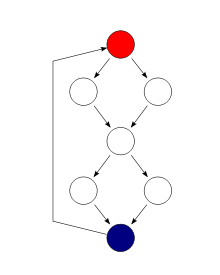
\includegraphics[width=0.5\textwidth]{../includes/pics/ciclomatica.png}
\end{center}
Tale indice può essere applicato a metodi, moduli e \markg{packages} di un programma per limitare la complessità durante lo sviluppo. Durante la fase dei test è possibile utilizzare l'indice per determinare il numero di test necessari in quanto fornisce un limite superiore da non eccedere.
\begin{itemize}
	\item \textbf{Range accettazione}: [0 - 30];
	\item \textbf{Range ottimale}: [0 - 10].
\end{itemize}
\subsubsection{Numero di metodi}
Questa metrica calcola la media di occorrenze di metodi per ciascun \markg{package} ed è utile poiché questi ultimi non dovrebbero contenere troppe definizioni di metodi. Un numero superiore alla media potrebbe indicare la necessità di una maggiore suddivisione del \markg{package} in questione.
\begin{itemize}
	\item \textbf{Range di accettazione}: [2 - 10];
	\item \textbf{Range ottimale}: [3 - 8].
\end{itemize}
\subsubsection{Variabili non utilizzate}
Il linguaggio \markg{Java} consente la creazione di variabili che possono non essere mai effettivamente utilizzare e quindi inutili. Questo tipo di variabili verrà individuato utilizzando un tool apposito chiamato \textit{ProGuard} che si occuperà anche di questo compito, fra i tanti altri oneri di ottimizzazione che gli spettano.
Non vi è nessun range di accettazione o alcun range ottimale da definire in quanto il valore di questa metrica deve sempre essere pari a 0.
\subsubsection{Numero di bug per linea}
Questa metrica è utile per quantificare il numero di bug presenti su una certa regione di codice, composta da un certo numero di linee. Rendendo il codice più chiaro e semplice possibile si ridurrà la probabilità di introdurre bug; il rischio di introdurre bug aumenta con il crescere del numero di righe di codice.
\begin{itemize}
	\item \textbf{Range di accettazione}: [0 - 60];
	\item \textbf{Range ottimale}: [0 - 25].
\end{itemize}
\subsubsection{Rapporto linee di codice e commento}
Questa metrica riguarda le linee di codice prodotte in rapporto con le linee di commento, escludendo le righe vuote. L'indicazione principale riguarda la manutenibilità del codice. Un rapporto troppo basso indica una carenza di informazioni necessarie alla comprensione del codice.
\begin{itemize}
	\item \textbf{Valore accettabile}: rapporto \textgreater { 0.20};
	\item \textbf{Valore ottimale}: rapporto \textgreater { 0.30}.
\end{itemize}
\subsection{Verifica}
\subsubsection{Descrizione}
In questa sezione verranno descritti gli strumenti ed i metodi impiegati per la \markg{verifica} del codice e dei documenti durante la loro realizzazione.
\subsubsection{Analisi statica}
L’analisi statica è una tecnica applicabile al codice ed alla documentazione che permette la \markg{verifica} di un prodotto individuandone gli errori. Può essere svolta secondo:
\begin{itemize}
	\item \textbf{Inspection}: si applica quando si ha un’idea delle possibili problematiche che si stanno cercando e si effettua facendo una comparazione tra il prodotto e una tabella di possibili errori creata in precedenza;
	\item \textbf{Walkthrough}: si applica quando non si sa quali sono le tipologie di errori che si stanno cercando. Occorre ispezionare tutto il codice o il documento per trovare qualsiasi tipo di anomalia.
\end{itemize}
\subsubsection{Analisi dinamica}
L’analisi dinamica consiste nella creazione ed esecuzione di una serie di test direttamente sul codice, utilizzando anche dei tool già realizzati appositamente per tali scopi. Non è possibile fare analisi dinamica sui documenti.
\subsubsection{Verifica diagrammi \markg{UML}}
I verificatori avranno il compito di controllare tutti i diagrammi \markg{UML} ed assicurarsi che rispettino lo standard \markg{UML}.
\subsubsection{Strumenti}
\begin{itemize}
	\item \textbf{Software}:  per la stesura del codice \markg{Java}, si utilizzeranno gli \markg{IDE} \emph{Intellij IDEA} e \emph{Android Studio};
	\item \textbf{Documenti}: per il controllo dei documenti verranno utilizzate le funzioni integrate a \markg{TexStudio} per controllare che non ci siano errori nei file \markg{LaTeX}. Verrà utilizzato GlossaryHelper per la gestione del glossario e per controllare che non vi siano presenti duplicati;
	\item \textbf{Gestione di \markg{processi} e \markg{feedback}}: verrà utilizzato il sistema di issues di \markg{GitLab};
	\item \textbf{Gestione di tasklist}: si utilizzeranno le funzionalità di Task Management di \markg{Asana};
	\item \textbf{Gestione del time tracking}: si utilizzeranno le funzionalità di Clockify (applicazione di time tracking free);
	\item \textbf{Analisi dinamica}: L'analisi dinamica sarà estesa a tutto il \markg{software} prodotto e consiste in test di unità tramite libreria di testing \markg{JUnit};
	\item \textbf{Tracciamento dei requisti}: verrà utilizzato lo un tool chiamato \emph{ProgmaDB} per tracciare i requisti installando lo strumento su un \markg{server} remoto condiviso.
\end{itemize}
\subsection{Validazione}
\subsubsection{Descrizione}
Il \markg{processo} di \markg{validazione} ha come scopo quello della \markg{verifica} del prodotto al fine di assicurarsi che sia conforme a quanto stabilito.
\subsubsection{Procedure}
L’attività di \markg{validazione} verrà svolta secondo i seguenti passi:
\begin{enumerate} 
	\item \textbf{Tracciamento}: tracciamento dei test con report da parte dei verificatori.
	\item \textbf{Analisi dei risultati}: in seguito al punto 1, spetterà al Responsabile di progetto l’analisi dei report e la decisione di:
	\begin{itemize}
		\item Accettare la \markg{validazione} e consegnare al proponente i risultati, informandolo sulle modalità di esecuzione della \markg{validazione};
		\item Ripetere i test in toto o in parte aggiungendo indicazioni mirate al miglioramento della fase di test che deve essere nuovamente eseguita.
	\end{itemize}
\end{enumerate}
